%%%%%%%%%%%%%%%%%%%%%%%%%%%%%%%%%%%%%%%%%%%%%%%%%%%%%%%%%%%%%%%%%%%%%%%%%%%%%%%%%%%%%%%%%
%%                                                                                     %%
%%                This file is part of the CAPH Compiler distribution                  %%
%%                            http:%/caph.univ-bpclermont.fr                           %%
%%                                                                                     %%
%%                                  Jocelyn SEROT                                      %%
%%                         Jocelyn.Serot@univ-bpclermont.fr                            %%
%%                                                                                     %%
%%         Copyright 2011-2018 Jocelyn SEROT.  All rights reserved.                    %%
%%  This file is distributed under the terms of the GNU Library General Public License %%
%%      with the special exception on linking described in file ..%LICENSE.            %%
%%                                                                                     %%
%%%%%%%%%%%%%%%%%%%%%%%%%%%%%%%%%%%%%%%%%%%%%%%%%%%%%%%%%%%%%%%%%%%%%%%%%%%%%%%%%%%%%%%%%

\chapter{Intermediate representation}
\label{chap:interm-repr}

\newcommand{\semr}[2]{#1\llbracket #2 \rrbracket}
\newcommand{\semtag}[3]{\mathsf{#2},#3,#1}
\newenvironment{code}
{\small\begin{alltt}}
{\end{alltt}\normalsize}

This chapter briefly describes the target-independant intermediate representation (IR) used as an input for the
back-ends.

The intermediate representation (IR) is basically a process network in
which each process is represented as a finite-state machine (FSM) and channels as
unbounded FIFOs.

Generation of this intermediate representation involves two steps : first generating a \emph{structural}
representation of the actor network and then generating a \emph{behavioral} description of each
actor involved in the network.

\section{Network generation}
\label{sec:network-generation}

Generating the structural representation of the actor network consists in instantiating each actor --
viewed as a black box at this level -- and ``wiring'' the resulting instances according to the
dependencies expressed by the functional definitions. This process is fully formalized by the static
semantics described in Chap.~\ref{chap:static}. The resulting network is set of \emph{boxes}
interconnected by \emph{wires}. Boxes result from the instanciation of actors and wires from the
data dependencies expressed in the definition section.

\section{Behavioral description}
\label{sec:behav-behav-descr}

Generating the behavioral description of an instantiated actor (box) consists in turning the set of
pattern-matching rules of the corresponding actor into a finite state machine with operations (FSMD
level). This process is depicted in Fig.~\ref{fig:box-fsm}. 

\begin{figure}[h]
\centering
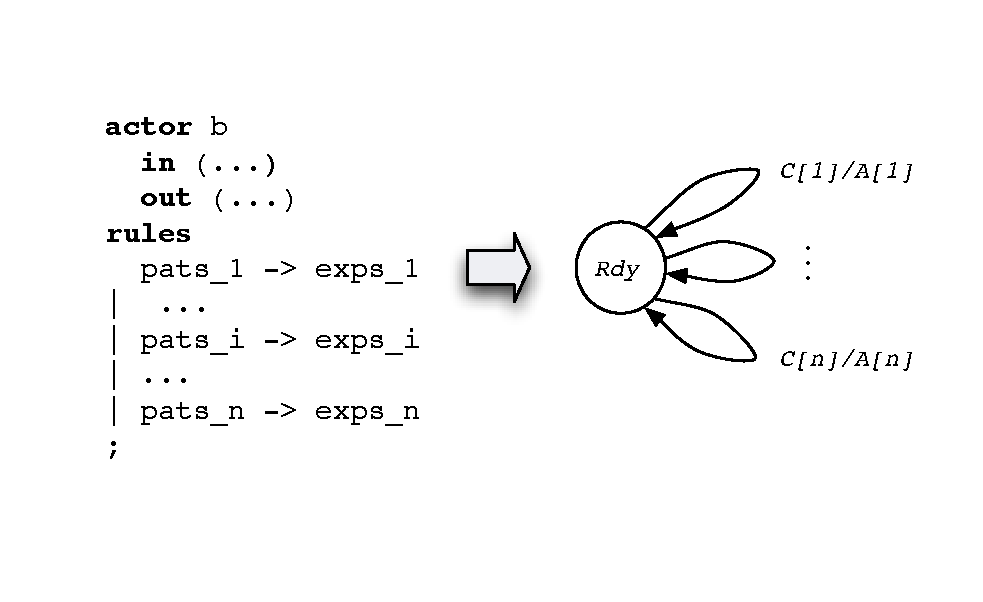
\includegraphics[width=0.85\linewidth]{figs/box-fsm}
\caption{Translation of a box into a FSM}
  \label{fig:box-fsm}�
\end{figure}  

At each rule $r_i$, consisting of a list of patterns $pats_i$ and a list of expressions $exps_i$, we
associate a set of \emph{conditions} $\semr{C}{r_i}$ and a set of actions $\semr{A}{r_i}$.
The set $\semr{C}{r_i}$ denotes the firing conditions for rule $r_i$, i.e. the conditions on the
  involved inputs, outputs and local variables that must be verified for the corresponding rule to be selected.
The set $\semr{A}{r_i}$ denotes the firing actions for rule $r_i$, i.e. the read operations and write
operations that must be performed on the involved inputs, outputs and variables when the corresponding rule is
selected.

\medskip
There are four possible firing conditions:
\begin{itemize}
\item $Avail_r(i)$, meaning that input $i$ is ready for reading (the connected FIFO is not empty),
\item $Match_i(i,pat)$ (resp.$Match_v(v,pat)$), meaning that input $i$ (resp. variable $v$) matches pattern $pat$,
\item $Avail_w(o)$, meaning that output $o$ is ready for writing (the connected FIFO is not full),
\item $Cond(exp)$, meaning that guard expression $exp$ (involving inputs and/or variables) is true
\end{itemize}
and four possible firing actions:
\begin{itemize}
\item $Read(i)$, meaning "read input $i$ (pop the corresponding from the connected FIFO)", ignoring
  the read value,
\item $Bind_i(i,pat)$, meaning "read input $i$ (pop the corresponding from the connected FIFO)
  and match the corresponding value against pattern $pat$", binding the variable(s) occurring in the
  pattern to the corresponding value(s),
\item $Bind_v(v,pat)$, meaning "match variable $v$ against pattern $pat$",
\item $Write_o(o,exp,\rho)$ (resp. $Write_v(v,exp,\rho)$), meaning "evaluate expression $exp$, using
  environment $\rho$ and write the resulting value on output $o$ (pushing the value on the connected
  FIFO) or in variable $v$.
\end{itemize}

Fig~\ref{fig:comp-rules} summarizes the rules for computing the sets $\semr{C}{r}$ and
$\semr{A}{r}$ from the patterns and expressions composing a rule. In these rules
$\_$ denotes the "empty" pattern (resp. expression), $const$ a constant pattern and $var$ a variable
pattern, $\txt{vars}(pat)$ is a function returning the name of all variables bound by a pattern and
$\rho_0$ is the ``default'' environment for evaluating a RHS expression, containing of the
values of the global and local variables.


\medskip
To illustrate the generation of the intermediate representation, let's take again the \texttt{suml} actor introduced in
Sec.~\ref{sec:actor-examples}. The code of this actor is given again below : 

\begin{lstlisting}[language=Caph,frame=single]
actor suml
  in (i:signed<16> dc)
  out (o:signed<16>)
var st : {S0,S1} = S0
var sum : int
rules 
  | (st:S0, i:'<) -> (sum:0, st:S1)
  | (st:S1, i:'>) -> (o:sum, st:S0)
  | (st:S1, i:'v) -> (sum:sum+v);
\end{lstlisting}

The corresponding intermediate representation is given in Fig.~\ref{fig:suml-fsm}. The small number appearing
beside each transition is the index of the corresponding rule.

\begin{figure}[h]
\centering
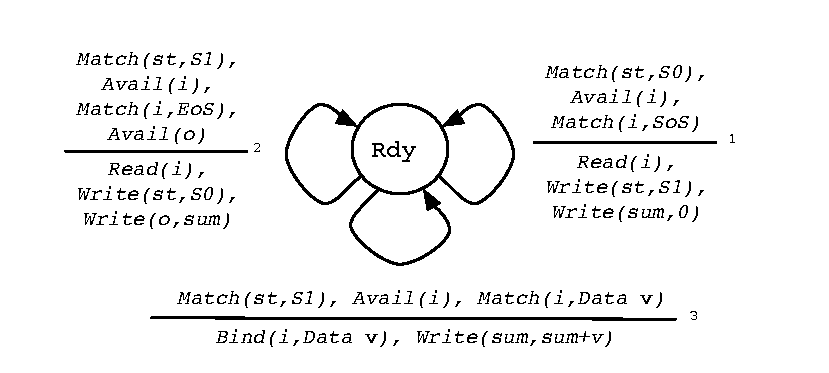
\includegraphics[width=0.75\linewidth]{figs/suml-fsm}
\caption{Intermediaire representation for the \texttt{suml} actor}
  \label{fig:suml-fsm}
\end{figure}  

\begin{figure}[t]
\begin{minipage}[b]{\textwidth}
\infrule[]
{\semr{C_r}{qpat_1,\ldots,qpat_m} =  C \andalso \semr{C_g}{gexp_1,\ldots,gexp_p} = C'' \andalso \semr{C_w}{qexp_1,\ldots,qexp_n} = C'}
{\semr{C}{qpat_1,\ldots,qpat_m\quad\mathtt{when}\quad gexp_1,\ldots,gexp_p\quad \rightarrow\quad
    qexp_1,\ldots,qexp_n} = C \cup C'' \cup C'}
\medskip
\infrule[]
{\semr{A_r}{qpat_1,\ldots,qpat_m} =  C, \rho \andalso \rho_0 \oplus \rho \vdash \semr{A_w}{qexp_1,\ldots,qexp_n} = A'}
{\semr{A}{qpat_1,\ldots,qpat_m \rightarrow qexp_1,\ldots,qexp_n} = A \cup A'}
\medskip
\infrule[]
{\forallin{i}{1}{m},~~ \semr{A_r}{qpat_i} = A_i, \rho_i}
{\semr{A_r}{qpat_1,\ldots,qpat_m} = \bigcup_{i=1}^{m}{A_i}, \C{i=1}{n}{\rho_i}}
\medskip
\infrule[]
{\forallin{i}{1}{n},~~ \rho \vdash \semr{A_w}{qexp_i} = A_i}
{\rho \vdash \semr{A_w}{qexp_1,\ldots,qexp_n} = \bigcup_{i=1}^{n}{A_i}}
\medskip
\begin{tabular}{rcl}
  $\semr{C_r}{qpat_1,\ldots,qpat_m} $ & $=$ & $ \bigcup_{j=1}^{m}{\semr{C'_r}{qpat_j}}$ \\ 
  $\semr{C_g}{gexp_1,\ldots,gexp_p} $ & $=$ & $ \bigcup_{j=1}^{p}{\semr{C''_r}{gexp_j}}$ \\ 
  $\semr{C_w}{qexp_1,\ldots,qexp_n} $ & $=$ & $ \bigcup_{j=1}^{n}{\semr{C'_w}{qexp_j}}$ \\ 
\\
  $\semr{C'_r}{\semtag{\_}{In}{i}} $ & $=$ & $ \emptyset$ \\
  $\semr{C'_r}{\semtag{pat}{In}{i}} $ & $=$ & $ \{ Avail_r(i), Match_i(i,pat) \}$ \\
  $\semr{C'_r}{\semtag{\_}{Var}{v}} $ & $=$ & $ \emptyset$ \\
  $\semr{C'_r}{\semtag{pat}{Var}{v}} $ & $=$ & $ \{ Match_v(v,pat) \}$ \\
\\
  $\semr{C'_w}{\semtag{\_}{Out}{o}} $ & $=$ & $ \emptyset$ \\
  $\semr{C'_w}{\semtag{exp}{Out}{o}} $ & $=$ & $ \{ Avail_w(o) \}$ \\
  $\semr{C'_w}{\semtag{exp}{Var}{v}} $ & $=$ & $ \emptyset$ \\
\\
  $\semr{C''_r}{exp} $ & $=$ & $ \{ Cond(exp) \}$ \\
\\
  $\semr{A'_r}{\semtag{\_}{In}{i}} $ & $=$ & $ \emptyset, \emptyset$ \\
  $\semr{A'_r}{\semtag{const}{In}{i}} $ & $=$ & $ \{ Read(i) \}, \emptyset$ \\
  $\semr{A'_r}{\semtag{pat}{In}{i}} $ & $=$ & $ \{ Bind_i(i,pat) \}, \text{vars}(pat)$ \\
  $\semr{A'_r}{\semtag{\_}{Var}{v}} $ & $=$ & $ \emptyset, \emptyset$ \\
  $\semr{A'_r}{\semtag{const}{Var}{v}} $ & $=$ & $ \emptyset, \emptyset$ \\
  $\semr{A'_r}{\semtag{var\ v}{Var}{v}} $ & $=$ & $ \emptyset, \emptyset$ \\
  $\semr{A'_r}{\semtag{pat}{Var}{v}} $ & $=$ & $ \{ Bind_v(v,pat) \}, \text{vars}(pat)$ \\
\\
  $\rho \vdash \semr{A'_w}{\semtag{\_}{Out}{o}} $ & $=$ & $ \emptyset$ \\
  $\rho \vdash \semr{A'_w}{\semtag{exp}{Out}{o}} $ & $=$ & $ \{ Write_o(o,exp,\rho) \}$ \\
  $\rho \vdash \semr{A'_w}{\semtag{\_}{Var}{v}} $ & $=$ & $ \emptyset$ \\
  $\rho \vdash \semr{A'_w}{\semtag{var\ v}{Var}{v}} $ & $=$ & $ \emptyset$ \\
  $\rho \vdash \semr{A'_w}{\semtag{exp}{Var}{v}} $ & $=$ & $ \{ Write_v(v,exp,\rho) \}$ \\
\end{tabular}
\end{minipage}
\caption{Rules for computing the $C$ and $A$ sets for actor rules}
\label{fig:comp-rules}
\end{figure}

%%% Local Variables: 
%%% mode: latex
%%% TeX-master: "caph"
%%% End: 
